\documentclass{zkdl-presentation-template}

\usepackage[T1]{fontenc}
\usepackage{kerkis}
\usepackage{kmath}
%\usepackage{concmath}
\usepackage{centernot}

\newcommand\leftarrowS{\leftarrow\joinrel\smalldollar}
\newcommand\rightarrowS{\smalldollar\joinrel\rightarrow}

\makeatletter
\newcommand{\smalldollar}{\mathrel{\mathpalette\small@dollar\relax}}
\newcommand{\small@dollar}[2]{%
  \vcenter{\hbox{%
    $#1\textnormal{\fontsize{0.7\dimexpr\f@size pt}{0}\selectfont\$}$%
  }}%
}
\makeatother

\tikzset{
    grid_cell/.style={
        rectangle, 
        draw=black, 
        very thick,
        minimum size=0.75cm, 
        font=\large\bfseries
    },
    grid_label/.style={
        font=\small
    },
    hypercube_highlight/.style={
        fill=gray!40
    }
}

\title[Sumcheck \& GKR]{\textbf{Sum-Check and GKR Protocols}}
\author{Distributed Lab}
\date{July 10, 2024}
\homepage{zkdl-camp.github.io}
\github{ZKDL-Camp}

\begin{document}
    \frame {
        \tikz [remember picture,overlay]
        \node at
            ([yshift=1.5cm,xshift=-1.5cm]current page.south east) 
            %or: (current page.center)
            {
\includegraphics[width=60pt]{images/logo.png}};
        \titlepage
    }
 
	\begin{frame}{Plan}
        \tableofcontents
    \end{frame}

	\section{Introduction}

    \begin{frame}{Recap on Poly-IOPs and NILPs}
        Almost all protocols we have seen so far work over \textbf{univariate
        $\mathbb{F}[X]$ polynomials}. \textit{Typical idea:} we aggregate
        information into some polynomial: say, $p(X)$ (which is typically a
        combination of other polynomials), and then check whether $p(u)=0$
        for every $u \in \Omega$:
        \begin{equation*}
            p(u) = 0 \; \text{for all} \; u \in \Omega \iff 
            p(X) = q(X)\prod_{u \in \Omega}(X-u)
        \end{equation*}

        We check this inequality at a random point $r \leftarrowS \mathbb{F}$
        and achieve soundness of $1-\deg p/|\mathbb{F}|$: see
        \textbf{Schwartz-Zippel Lemma}.

        For appropriate domains (typically $\Omega = \{\omega^j\}_{j \in
        [2^t]}$) we reduce all polynomials computations to $\mathcal{O}(n\log
        n)$ complexity.

        \begin{block}{Motivation}
            But what if we could work with much smaller degrees?
        \end{block}
    \end{frame}

    \begin{frame}{Sum-Check Protocols}
        \begin{itemize}
            \item Instead of $n$-variate univariate polynomials $\mathbb{F}[X]$
            we reduce the problem to $\log n$-variate multivariate polynomials
            $\mathbb{F}[X_1,\dots,X_v]$.
            \item The Schwartz-Zippel Lemma still holds for multivariate case:
            \begin{equation*}
                \mathop{\text{Pr}}_{(r_1,\dots,r_v) \leftarrowS \mathbb{S}}[f(r_1,\dots,r_v) = 0] \leq \frac{\deg f}{|\mathbb{S}|}, \quad \mathbb{S} \subseteq \mathbb{F}^v
            \end{equation*}
            \item \textbf{Bad news:} divisibility theorems do not hold:
            \begin{equation*}
                f(s_1,\dots,s_v) = 0 \centernot\iff (X-s_1)\dots (X-s_v) \mid f(X_1,\dots,X_v)
            \end{equation*}
        \end{itemize}

        \begin{alertblock}{Sum-Check meaning}
            Instead of divisibility checks, we use the \textbf{Sum-Check}:
            \begin{equation*}
                \sum_{b_1 \in \{0,1\}}\sum_{b_2 \in \{0,1\}}\dots \sum_{b_v \in \{0,1\}} f(b_1,\dots,b_v) = H
            \end{equation*}
        \end{alertblock}
    \end{frame}

    \begin{frame}{Summary in a Nutshell}
        \begin{figure}
            \centering
            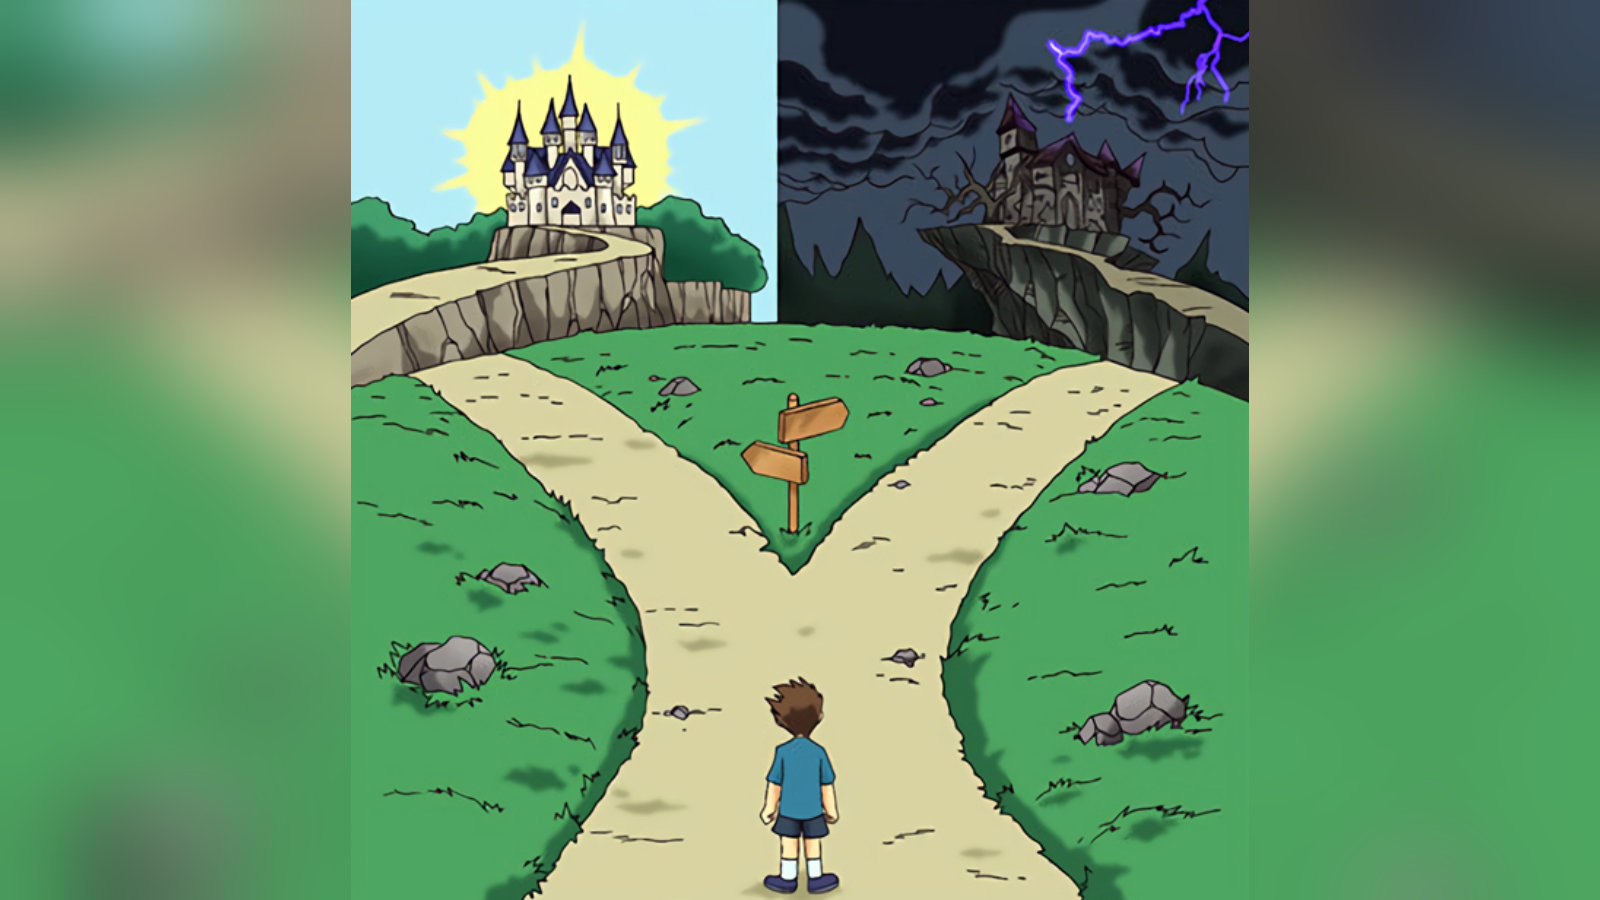
\includegraphics[width=0.65\textwidth]{images/lecture_15/bad_boy.jpg}
        \end{figure}
        \begin{columns}
            \begin{column}{0.5\textwidth}
                \textcolor{blue!70!black}{\begin{center}
                    \textbf{Univariate World:}
                \end{center}
                \[p(X) = q(X)\prod_{u \in \Omega}(X-u)\]}
            \end{column}
            \begin{column}{0.5\textwidth}
                \textcolor{green!50!black}{
                \begin{center}
                    \textbf{Multivariate World:}
                \end{center}
                \[\sum_{\mathbf{b} \in \{0,1\}^{\ell}} f(b_1,\dots,b_{\ell}) = H\]}
            \end{column}
        \end{columns}

        \vspace{-10px}
        
        \textbf{Succinct Arguments:} Ligero (2022), Spartan (2020), Libra
        (2019), Hyrax(2017), GKR (2008), \dots

        \textbf{Applications:} zkGPT (2025), deep-prove (using \textit{Ceno})
        (2024), vSQL (2017), \dots
    \end{frame}

    \section{Multivariate Polynomials. Multilinear Extensions.}

    \begin{frame}{Some technicalities}
        \begin{definition}[Monomial]
            By \textbf{monomial} in $v$ variables we call expression
            $\mu(\mathbf{X})=X_1^{\alpha_1}\dots X_v^{\alpha_v}$ where
            $\alpha_1,\dots,\alpha_v$ are non-negative integers. The
            \textbf{degree} of a monomial is naturally defined as $\deg \mu \triangleq
            \alpha_1+\dots+\alpha_v$.
        \end{definition}

        \begin{definition}[Multivariate Polynomial]
            Function $f: \mathbb{F}^v \to \mathbb{F}$ is called an
            \textbf{$v$-variate polynomial}, which is denoted by $f \in
            \mathbb{F}[X_1,\dots,X_v]$, if $f(\mathbf{X})$ is a finite linear
            combination of $v$-variate monomials
            $\{\mu_1(\mathbf{X}),\dots,\mu_n(\mathbf{X})\}$. The \textbf{degree}
            of $f$ is defined as $\deg f \triangleq \max_{i \in \{1,\dots,n\}}
            \deg \mu_i$. 
        \end{definition}

        \begin{example}
            $f(X_1,X_2,X_3)=X_1^3 + 3X_1^2X_2^2 + X_3^2 + X_3$ is a linear
            combination of 3-variate monomials $\{X_1^3, X_1^2X_2^2, X_3^2,
            X_3\}$, thus $f \in \mathbb{F}[X_1,X_2,X_3]$. It has degree $\deg
            f=4$, corresponding to the second monomial $X_1^2X_2^2$.
        \end{example}
    \end{frame}

    \begin{frame}{Multilinear Polynomials}
        \begin{definition}[Multilinear Polynomial]
            Multivariate polynomial $f \in \mathbb{F}[X_1,\dots,X_v]$ is called
            \textbf{multilinear} if it is linear in each of the variables.
            Formally we have:
            \begin{equation*}
                f(X_1,\dots,X_v) = \textcolor{red}{\alpha_j} X_j + \textcolor{blue}{\beta_j}, \quad j \in \{1,\dots,n\},
            \end{equation*}
            where $\alpha_j,\beta_j$ do not depend on $X_j$.
        \end{definition}

        \begin{example}
            For example, $f(X_1,X_2,X_3) = X_1X_2 + 3X_1X_3 + X_2X_3$ is a multilinear 
            polynomial in $3$ variables. For instance, for $X_1$:
            \begin{equation*}
                f(X_1,X_2,X_3) = \textcolor{red}{(X_2+3X_3)}X_1 + \textcolor{blue}{X_2X_3}.
            \end{equation*}

            Similarly, $f(X_1,\dots,X_v)=\prod_{i=1}^v X_i$ is a multilinear
            polynomial.
        \end{example}
    \end{frame}

    \begin{frame}{Boolean Hypercube}
        \begin{definition}[Boolean Hypercube]
            By \textbf{$v$-dimensional boolean hypercube} we simply denote the
            set $\{0,1\}^v$ (which is a set of binary strings of length $v$). 
        \end{definition}

        \begin{figure}
            \centering
            
\includegraphics[width=0.65\textwidth]{images/lecture_15/meme.jpg}
            \caption{Cryptographers \textit{love} overcomplicating things.}
        \end{figure}
    \end{frame}

    \begin{frame}{Multilinear Extensions (MLE)}
        \begin{definition}[Boolean Hypercube Extension]
            Suppose we are given the values on the boolean cybercube $f:
            \{0,1\}^v \to \mathbb{F}$. We call $\widetilde{f}: \mathbb{F}^v \to
            \mathbb{F}$ an \textbf{extension} if $\widetilde{f}(\mathbf{b}) =
            f(\mathbf{b})$ for every $\mathbf{b} \in \{0,1\}^v$.
        \end{definition}

        \begin{center}
    % We scale the TikZ picture to fit the frame width nicely
    \resizebox{0.95\textwidth}{!}{
        \begin{tikzpicture}
            %===========================================================
            % LEFT GRID: Function on the Boolean Hypercube {0,1}^2
            %===========================================================
            
            \node[grid_label, below=0.75cm of {(-0.6, -0.5)}] (title_f) {Function $f: \{0,1\}^2 \to \mathbb{F}$};
            
            % --- Draw the grid nodes ---
            \node[grid_cell] (f11) at (0,0) {3};
            \node[grid_cell] (f10) at (0,-0.75) {2};
            \node[grid_cell] (f01) at (-0.75,0) {2};
            \node[grid_cell] (f00) at (-0.75,-0.75) {1};
            
            % --- Draw the labels for the grid ---
            % X-axis labels
            \node[grid_label, above=0.1cm of f01] {$0$};
            \node[grid_label, above=0.1cm of f11] {$1$};
            % Y-axis labels
            \node[grid_label, left=0.1cm of f01] {$1$};
            \node[grid_label, left=0.1cm of f00] {$0$};
            
            
            %===========================================================
            % Arrow in the middle
            %===========================================================
            \draw[->, ultra thick] (1.2, -0.6) -- node[above, font=\large] {Extend} (2.8, -0.6);
            
            
            %===========================================================
            % RIGHT GRID: Extension over the larger field F_5
            %===========================================================
            
            \node[grid_label, align=center, below=0.2cm of {(5.5, -3.25)}] (title_f_tilde) {Extension $\widetilde{f}: \mathbb{F}_5^2 \to \mathbb{F}_5$ \\ $\widetilde{f}(X_1, X_2) = X_1^2 + X_2^2 + 1$};
            
            % --- Draw the grid nodes with calculated values ---
            \foreach \x in {0,...,4} {
                \foreach \y in {0,...,4} {
                    \pgfmathparse{int(mod(\x*\x + \y*\y + 1, 5))}
                    \let\value\pgfmathresult
                    
                    \ifnum\x<2
                        \ifnum\y<2
                            \node[grid_cell, hypercube_highlight] at ({4+\x*0.75}, {-\y*0.75}) {\value};
                        \else
                            \node[grid_cell] at ({4+\x*0.75}, {-\y*0.75}) {\value};
                        \fi
                    \else
                        \node[grid_cell] at ({4+\x*0.75}, {-\y*0.75}) {\value};
                    \fi
                }
            }
            
            % --- Draw the labels for the 5x5 grid ---
            \foreach \x in {0,...,4} {
                \node[grid_label, above=0.1cm of {({4+\x*0.75}, 0.3)}] {$\x$};
            }
            \foreach \y in {0,...,4} {
                \node[grid_label, left=0.1cm of {({3.6}, {-\y*0.75})}] {$\y$};
            }
        
        \end{tikzpicture}
    }
    \end{center}
    
    \end{frame}

    \begin{frame}[plain, standout]
        \centering
        \LARGE
        \textbf{Thank you for your attention} \\
        
        \vspace{0.2cm} \Huge \ding{170} \large \\
        
        \vspace{1cm}
  
        \href{https://zkdl-camp.github.io/}{\raisebox{-.1em}{\hspace{.025em}\faIcon{globe}}\hspace{.325em}zkdl-camp.github.io} \\
  
        \href{https://github.com/ZKDL-Camp}{\raisebox{-.1em}{\hspace{.025em}\faIcon{github}}\hspace{.325em}github.com/ZKDL-Camp}
        
        \begin{center}
            
\includegraphics[width=0.15\textwidth]{images/logo.png}
        \end{center}
    \end{frame}
\end{document}
